% This file was created with tikzplotlib v0.10.1.
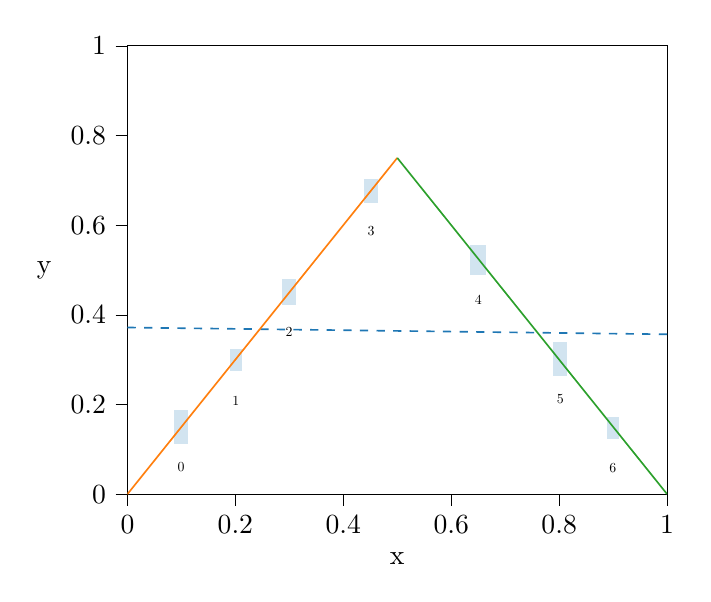
\begin{tikzpicture}

\definecolor{darkgray176}{RGB}{176,176,176}
\definecolor{darkorange25512714}{RGB}{255,127,14}
\definecolor{forestgreen4416044}{RGB}{44,160,44}
\definecolor{steelblue31119180}{RGB}{31,119,180}

\begin{axis}[
tick align=outside,
tick pos=left,
x grid style={darkgray176},
xlabel={x},
xmin=0, xmax=1,
xtick style={color=black},
y grid style={darkgray176},
ylabel style={rotate=-90.0},
ylabel={y},
ymin=0, ymax=1,
ytick style={color=black}
]
\draw[draw=none,fill=steelblue31119180,fill opacity=0.2] (axis cs:0.0863549312885544,0.111078793138061) rectangle (axis cs:0.112806198011638,0.188434497040419);
\draw[draw=none,fill=steelblue31119180,fill opacity=0.2] (axis cs:0.189375164539954,0.27412048464376) rectangle (axis cs:0.211987961843501,0.323325474043981);
\draw[draw=none,fill=steelblue31119180,fill opacity=0.2] (axis cs:0.286093458968633,0.422091543203351) rectangle (axis cs:0.312554964908266,0.480213394695103);
\draw[draw=none,fill=steelblue31119180,fill opacity=0.2] (axis cs:0.439086533207921,0.648839255430186) rectangle (axis cs:0.464267564376244,0.703591376671839);
\draw[draw=none,fill=steelblue31119180,fill opacity=0.2] (axis cs:0.635223140536826,0.488398611886978) rectangle (axis cs:0.664921067341259,0.556247871429456);
\draw[draw=none,fill=steelblue31119180,fill opacity=0.2] (axis cs:0.789036495130863,0.263382233795743) rectangle (axis cs:0.814853975506851,0.339938585821692);
\draw[draw=none,fill=steelblue31119180,fill opacity=0.2] (axis cs:0.888825958226993,0.123348423896125) rectangle (axis cs:0.910131769242549,0.17182016252774);
\addplot [semithick, steelblue31119180, dashed]
table {%
0 0.371672987937927
1.01010096073151 0.356310248374939
};
\addplot [semithick, darkorange25512714]
table {%
0 0
0.5 0.75
};
\addplot [semithick, forestgreen4416044]
table {%
0.5 0.75
1 -0
};
\draw (axis cs:0.0995805646500963,0.0497566450892399) node[
  scale=0.5,
  anchor=base,
  text=black,
  rotate=0.0
]{0};
\draw (axis cs:0.200681563191727,0.19872297934387) node[
  scale=0.5,
  anchor=base,
  text=black,
  rotate=0.0
]{1};
\draw (axis cs:0.299324211938449,0.351152468949227) node[
  scale=0.5,
  anchor=base,
  text=black,
  rotate=0.0
]{2};
\draw (axis cs:0.451677048792083,0.576215316051012) node[
  scale=0.5,
  anchor=base,
  text=black,
  rotate=0.0
]{3};
\draw (axis cs:0.650072103939042,0.422323241658217) node[
  scale=0.5,
  anchor=base,
  text=black,
  rotate=0.0
]{4};
\draw (axis cs:0.801945235318857,0.201660409808718) node[
  scale=0.5,
  anchor=base,
  text=black,
  rotate=0.0
]{5};
\draw (axis cs:0.899478863734771,0.0475842932119327) node[
  scale=0.5,
  anchor=base,
  text=black,
  rotate=0.0
]{6};
\end{axis}

\end{tikzpicture}
